% ************************************************************************* %
% ********************** MTCONNECT DOCUMENT TEMPLATE ********************** %
% ************************************************************************* %
% 	FILENAME: 		mtconnect.tex											%
%	VERSION:		0.1														%
% 	DATE:			02/13/2018												%
%	PORTED BY:		Moneer Helu												%
%	ADDRESS:		Engineering Laboratory									%
%					National Institute of Standards and Technology (NIST)	%
%					100 Bureau Drive										%
%					Mailstop 8260											%
%					Gaithersburg, MD 20899									%
%					United States of America								%
% 	EMAIL:			moneer.helu@nist.gov									%
% 	DESCRIPTION:	Template for MTConnect documentation;					%
% 					Initial attempt for testing and discussion				%
% 	USAGE:			\documentclass[options]{mtconnect}						%
% ************************************************************************* %

\documentclass{mtconnect}	% Load mtconnect document class

\begin{document}			% Begin document here

% ************************************************************************* %
% *********************** REQUIRED INITIAL INPUTS ************************* %
% ************************************************************************* %

\docnum{OPC/UA}							% Document "number"
\doctitle{\mtconnect and OPC/UA Companion Specification}	% Full document title
\doctitleshort{\mtconnect OPC/UA Companion Specification}				% Shortened document title
\versionnum{2.0}						% MTConnect version
\preparedfor{MTConnect Institute and OPC Foundation}		% Should not change!!!
\preparedby{List of authors\ldots}				% Author
\preparedon{September 29, 2018}			% Date prepared
\drafttext{Draft }

% ************************************************************************* %
% ******************* FRONT MATTER (DO NOT CHANGE!!!) ********************* %
% ************************************************************************* %

\begin{nolinenumbers}
	\maketitle				% Title page
\end{nolinenumbers}

\pagenumbering{roman}

% MTConnect Specification and Material Statement:
\textbf{\color{mtc1}\Large {OPC Foundation and \mtconnect Institute}}

\begin{center}
    \textbf{AGREEMENT OF USE}
\end{center}

\textbf{COPYRIGHT RESTRICTIONS}

\begin{itemize}
    \item This document is provided "as is" by the OPC Foundation and the MTConnect Institute.
    \item Right of use for this specification is restricted to this specification and does not grant rights of use for referred documents.
    \item Right of use for this specification will be granted without cost.
    \item This document may be distributed through computer systems, printed or copied as long as the content remains unchanged and the document is not modified.
    \item OPC Foundation and the MTConnect Institute do not guarantee usability for any purpose and shall not be made liable for any case using the content of this document.
    \item The user of the document agrees to indemnify OPC Foundation and the MTConnect Institute and their officers, directors and agents harmless from all demands, claims, actions, losses, damages (including damages from personal injuries), costs and expenses (including attorneys' fees) which are in any way related to activities associated with its use of content from this specification.
    \item The document shall not be used in conjunction with company advertising, shall not be sold or licensed to any party.
    
    \item The intellectual property and copyright is solely owned by the OPC Foundation and the MTConnect Institute.
\end{itemize}

\textbf{PATENTS} 

The attention of adopters is directed to the possibility that compliance with or adoption of OPC or the MTConnect Institute specifications may require use of an invention covered by patent rights. OPC Foundation or the MTConnect Institute shall not be responsible for identifying patents for which a license may be required by any OPC or the MTConnect Institute specification, or for conducting legal inquiries into the legal validity or scope of those patents that are brought to its attention. OPC or the MTConnect Institute specifications are prospective and advisory only. Prospective users are responsible for protecting themselves against liability for infringement of patents.

\textbf{WARRANTY AND LIABILITY DISCLAIMERS}

WHILE THIS PUBLICATION IS BELIEVED TO BE ACCURATE, IT IS PROVIDED "AS IS" AND MAY CONTAIN ERRORS OR MISPRINTS. THE OPC FOUDATION NOR THE MTCONNECT INSTITUTE MAKES NO WARRANTY OF ANY KIND, EXPRESSED OR IMPLIED, WITH REGARD TO THIS PUBLICATION, INCLUDING BUT NOT LIMITED TO ANY WARRANTY OF TITLE OR OWNERSHIP, IMPLIED WARRANTY OF MERCHANTABILITY OR WARRANTY OF FITNESS FOR A PARTICULAR PURPOSE OR USE. IN NO EVENT SHALL THE OPC FOUNDATION NOR THE MTCONNECT INSTITUTE BE LIABLE FOR ERRORS CONTAINED HEREIN OR FOR DIRECT, INDIRECT, INCIDENTAL, SPECIAL, CONSEQUENTIAL, RELIANCE OR COVER DAMAGES, INCLUDING LOSS OF PROFITS, REVENUE, DATA OR USE, INCURRED BY ANY USER OR ANY THIRD PARTY IN CONNECTION WITH THE FURNISHING, PERFORMANCE, OR USE OF THIS MATERIAL, EVEN IF ADVISED OF THE POSSIBILITY OF SUCH DAMAGES.

The entire risk as to the quality and performance of software developed using this specification is borne by you. 

\textbf{RESTRICTED RIGHTS LEGEND}

This Specification is provided with Restricted Rights. Use, duplication or disclosure by the U.S. government is subject to restrictions as set forth in (a) this Agreement pursuant to DFARs 227.7202-3(a); (b) subparagraph (c)(1)(i) of the Rights in Technical Data and Computer Software clause at DFARs 252.227-7013; or (c) the Commercial Computer Software Restricted Rights clause at FAR 52.227-19 subdivision (c)(1) and (2), as applicable. Contractor / manufacturer are the OPC Foundation, 16101 N. 82nd Street, Suite 3B, Scottsdale, AZ, 85260-1830

\textbf{COMPLIANCE}

The combination of the MTConnect Institute and OPC Foundation shall at all times be the sole entities that may authorize developers, suppliers and sellers of hardware and software to use certification marks, trademarks or other special designations to indicate compliance with these materials as specified within this document. Products developed using this specification may claim compliance or conformance with this specification if and only if the software satisfactorily meets the certification requirements set by the MTConnect Institute or the OPC Foundation. Products that do not meet these requirements may claim only that the product was based on this specification and must not claim compliance or conformance with this specification. 

\textbf{TRADEMARKS}

Most computer and software brand names have trademarks or registered trademarks. The individual trademarks have not been listed here.

\textbf{GENERAL PROVISIONS}

Should any provision of this Agreement be held to be void, invalid, unenforceable or illegal by a court, the validity and enforceability of the other provisions shall not be affected thereby. 

This Agreement shall be governed by and construed under the laws of Germany.
This Agreement embodies the entire understanding between the parties with respect to, and supersedes any prior understanding or agreement (oral or written) relating to, this specification.


\clearpage
\tableofcontents
\thispagestyle{fancy}
\clearpage
\listoffigures
\thispagestyle{fancy}
\clearpage
%\listoftables
%\clearpage
\pagenumbering{arabic}

% ************************************************************************* %
% ******************** ENTER DOCUMENT CONTENT BELOW *********************** %
% ************************************************************************* %

\section{Introduction}\label{intro}

\subsection{Background}

In September 2010, the OPC Foundation and the MTConnect Institute signed a memorandum of understanding to provide a mechanism for OPC and MTConnect to collaborate to extend the reach of the existing manufacturing data exchange standards and implementation technologies in order to:

\begin{itemize}
    \item Evolve the existing standards for each organization to provide complete manufacturing technology interoperability.
    \item Provide the mechanism for continuous improvement of standards and specifications overseen by each body.
    \item Work directly with the end users and suppliers of technology and manufacturing. 
    \item Provide a coordinating function to exchange insights, identify overlaps, and harmonize work where appropriate.
    \item Facilitate clear communication and education for users and others concerning possible overlaps and the ways the standards and specifications can be used.
    \item Provide a solid foundation to develop and deliver specifications, technology and processes to facilitate adoption of the technology into real products.
\end{itemize}

The outcome of that agreement was an initial companion specification called MTConnect-OPC UA Version 1.2.0. MTConnect-OPC UA companion specification describes an architecture for exchanging information for interoperability and consistency between MTConnect specifications and the OPC Unified Architecture (UA) specifications, as well as describing the manufacturing technology equipment, devices, software or other products that may implement those standards.

This document, OPC Unified Architecture for MTConnect Companion Specification Draft Version 2.0, provides an update to the original companion specification to include the latest capabilities and functionality of the standards provided by the MTConnect Institute and the OPC Foundation.

\subsection{MTConnect-OPC UA Goals}

The OPC Unified Architecture for MTConnect Companion Specification is designed with the following goals in mind, in the interest of wide and rapid adoption by vendors of equipment and software:

\begin{itemize}
    \item Incremental adoption:the technical barrier to MTConnect-OPC UA enablement will be greatly reduced with this companion specification and the source code and binaries available in the MTConnect-OPC UA reference port.
    \item Evolution: MTConnect and OPC UA can incrementally evolve without jeopardizing backwards compatibility of previous MTConnect-OPC UA versions.
    \item Customizability: MTConnect-OPC UA's extensibility enables integrators to create value-added software and tools that are machine-specific or installation-specific, without jeopardizing compatibility with other equipment or software.
    \item Non-proprietary: built on open standards, backed by both the OPC Foundation and the MTConnect Institute which represents hundreds of companies, individuals, government organizations and non-profits all working toward the goal of increased productivity in the manufacturing arena.
\end{itemize}

\subsection{Who Will Find Benefit from this Specification?}

To adopt the OPC Unified Architecture for MTConnect Companion Specification one will need to have a clear understanding of both MTConnect and OPC UA. From the technical side, we will discuss MTConnect-OPC UA from:

\begin{itemize}
    \item The backend or OPC UA Server and MTConnect agent/adapter architecture.
    \item The client or software application side, we will discuss how one develops an application that is MTConnect-OPC UA enabled.
    \item Applying MTConnect semantics to devices containing an embedded OPC UA Server.
\end{itemize}

From the business side, we will reference a companion business MTConnect-OPC UA white paper that addresses the concerns from the owners and top management of the business as well as the operations and engineering management. It is the objective of this white paper to provide information primarily to MTConnect and OPC UA software developers. We do not make assumptions about the level of programming expertise beyond what would be considered to be "reasonable" level of expertise. It is for this reason that we include enough details about both MTConnect and OPC UA to provide the ability to implement this companion specification without having references back to other documents. However, the OPC and MTConnect standards are critical and become much more meaningful with the appropriate overview from this document.

\subsection{References}

\subsubsection{OPC Foundation}

The following specifications from the OPC foundation are referenced by this specification.

\hang [UA Part 1]	OPC UA Specification: Part 1 -- Concepts \\
\url{http://www.opcfoundation.org/UA/Part1/}\label{doc:UA_Part_1}

\hang [UA Part 2]	OPC UA Specification: Part 2 -- Security Model \\
\url{http://www.opcfoundation.org/UA/Part2/}

\hang [UA Part 3]	OPC UA Specification: Part 3 -- Address Space Model \\
\url{http://www.opcfoundation.org/UA/Part3/}

\hang [UA Part 4]	OPC UA Specification: Part 4 -- Services \\
\url{http://www.opcfoundation.org/UA/Part4/}

\hang [UA Part 5]	OPC UA Specification: Part 5 -- Information Model \\
\url{http://www.opcfoundation.org/UA/Part5/}

\hang [UA Part 6]	OPC UA Specification: Part 6 -- Mappings \\
\url{http://www.opcfoundation.org/UA/Part6/}

\hang [UA Part 7]	OPC UA Specification: Part 7 -- Profiles \\
\url{http://www.opcfoundation.org/UA/Part7/}

\hang [UA Part 8]	OPC UA Specification: Part 8 -- Data Access \\
\url{http://www.opcfoundation.org/UA/Part8/}

\hang [UA Part 9]	OPC UA Specification: Part 9 -- Alarms and Conditions \\
\url{http://www.opcfoundation.org/UA/Part9/}

\hang [UA Part 10]	OPC UA Specification: Part 10 -- Programs \\
\url{http://www.opcfoundation.org/UA/Part10/}

\hang [UA Part 11]	OPC UA Specification: Part 11 -- Historical Access \\
\url{http://www.opcfoundation.org/UA/Part11/}

\hang [UA Part 13]	OPC UA Specification: Part 13 -- Aggregates \\
\url{http://www.opcfoundation.org/UA/Part13/}

\subsubsection{\mtconnect Institute}

\hang [MT Part 1.0]	\mtconnect Standard: Part 1.0 -- Overview and Fundamentals, Version 1.4.0 \\
\url{https://static1.squarespace.com/static/54011775e4b0bc1fe0fb8494/t/5acb81f96d2a73d3a01281c5/1523286521969/MTC_Part1_0_OverviewAndFundamentals1_4_0.pdf}

\hang [MT Part 2.0]	\mtconnect Standard: Part 2.0 -- Devices Information Model, Version 1.4.0 \\
\url{https://static1.squarespace.com/static/54011775e4b0bc1fe0fb8494/t/5acb822e352f53a44f10534b/1523286575786/MTC_Part2_0_Devices_1_4_0.pdf}

\hang [MT Part 3.0]	\mtconnect Standard: Part .0 -- Streams Information Model, Version 1.4.0 \\
\url{https://static1.squarespace.com/static/54011775e4b0bc1fe0fb8494/t/5acb651e88251b53486ed7f5/1523279135088/MTC_Part3_0_StreamsInformationModel_1_4_0.pdf}

\hang [MT Part 4.0	\mtconnect Standard: Part 4 -- Assets Information Model, Version 1.4.0 \\
\url{https://static1.squarespace.com/static/54011775e4b0bc1fe0fb8494/t/5acb824a8a922dc773e19caf/1523286602677/MTC_Part4_0_AssetsInformationModel_1_4_0.pdf}

\hang [MT Part 4.1]	\mtconnect Standard: Part 4.1 -- Cutting Tools, Version 1.4.0 \\
\url{https://static1.squarespace.com/static/54011775e4b0bc1fe0fb8494/t/5acb825a03ce649b2a64b282/1523286619088/MTC_Part4_1_CuttingTools_1_4_0.pdf}

\hang [MT Part 5.0]	\mtconnect Standard: Part 5.0 -- Interfaces, Version 1.4.0 \\
\url{https://static1.squarespace.com/static/54011775e4b0bc1fe0fb8494/t/5acb826a352f53a44f10606f/1523286635455/MTC_Part5_0_Interfaces_1_4_0.pdf}

\subsection{Abbrevations}

The following abbreviation are used in this document:

\begin{itemize}
    \item ERP -- Enterprise Resource Planning
    \item HMI -- Human Machine Interface
    \item HTTP -- Hyper Text Transport Protocol
    \item MES -- Management Execution Systems
    \item PLC -- Programmable Logic Controller
    \item PMS -- Production Management Systems
    \item SCADA -- Supervisory Control And Data Acquisition
    \item TCP/IP -- Transmission Control Protocol/Internet Protocol
    \item XML -- eXtensible Mark-up Language
\end{itemize}

\section{Use Cases}

\subsection{Overview}

Before delving into the details of the specification it is useful to identify some of the key use cases for the technology. The use cases defined here are not an exhaustive list; however, they should help demonstrate how this specification is expected to be used and to help illustrate the benefits of a common information model.

\subsection{Device Maker}

The use case, shown in Figure \ref{fig:device_mfg_use_case}, centers on the manufacturer of a piece of equipment or device that needs to provide connectivity to other systems. In some cases, the device manufacturer will be targeting markets other than equipment (Machine Tool) and would benefit from a more generic specification like OPC UA. On the other hand, the standardized semantics of MTConnect are extremely important to standardized communications on the manufacturing shop floor. The MTConnect-OPC UA specification and the resulting standard information model allows the device manufacturers to standardize on OPC UA as the network interface while making their information accessible to software applications that includes the enhanced meaning and structure provided by applying the MTConnect semantics. Figure 1 shows several clients developed for different purposes that can access information produced by the device via OPC UA.

\begin{figure}[h]
  \centering
  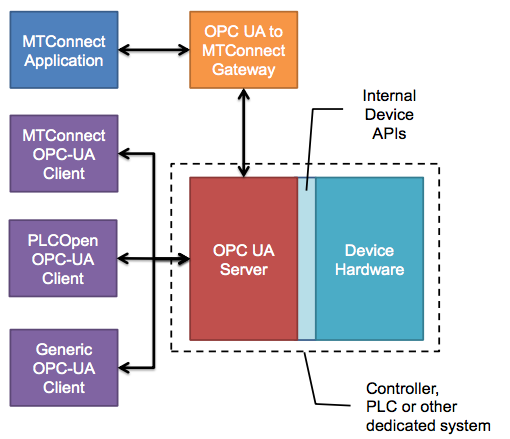
\includegraphics[width=0.75\textwidth]{diagrams/DeviceManufacturingUseCase.png}
  \caption{Device Manufacturer's Use Case}
  \label{fig:device_mfg_use_case}
\end{figure}

The device manufacture may also have a native MTConnect device and make use of an MTConnect to OPC UA gateway to provide the information to OPC UA aware clients (see Figure \ref{fig:device_mfg_native} and Figure \ref{fig:device_mfg_separate}). This standard allows for easy information flow between Client and Server that support either MTConnect or OPC UA.

The MTConnect or OPC UA interface may reside directly in the Machine, but it may also reside in some other device that communicates with the Machine. The actual location for the interface is up to the Machine vendor.

\textit{Should we add Minimum Level of OPC Functionality required to support this scenario}

\begin{figure}[h]
  \centering
  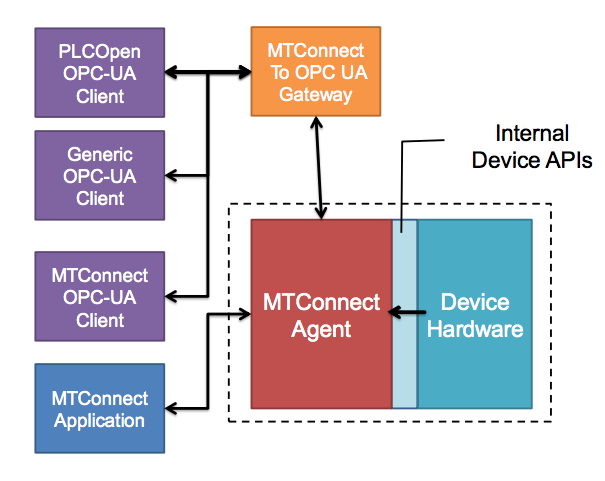
\includegraphics[width=0.75\textwidth]{diagrams/DeviceManufacturerNativeMTConnect.png}
  \caption{Device Manufacturer with Native MTConnect}
  \label{fig:device_mfg_native}
\end{figure}

\begin{figure}[h]
  \centering
  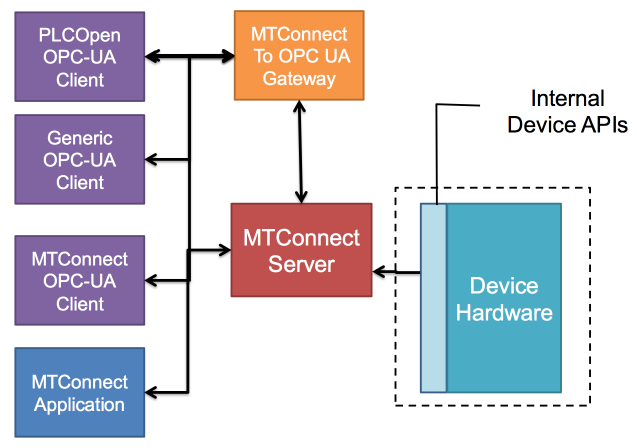
\includegraphics[width=0.75\textwidth]{diagrams/DeviceManufacturerSeparateAgent.png}
  \caption{Device Manufacturer with Separate MTConnect Agent}
  \label{fig:device_mfg_separate}
\end{figure}

\FloatBarrier

\subsubsection{Independent Software Vendor}

The use case shown in Figure \ref{fig:isv_use_case} centers on an Independent Software Vendor (ISV) that wishes to sell products to users of equipment such as Machine Tools. An ISV will typically want to provide gateways that convert information between MTConnect and OPC UA as well as adding numerous features that add value to the semantics defined in the MTConnect standards. The MTConnect-OPC UA specification allows the ISV to extend the MTConnect-OPC UA information model with application specific constructs which can be easily accessed via any standard OPC UA client product. These added features will exist in parallel to the standard MTConnect interfaces. Figure \ref{fig:isv_use_case} shows an ISV product that consumes data from MTConnect and OPC UA enabled devices and then makes it available via MTConnect and OPC UA.

\begin{figure}[h]
  \centering
  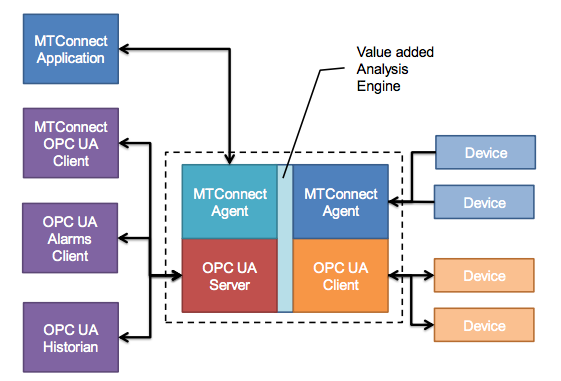
\includegraphics[width=0.75\textwidth]{diagrams/ISVUseCase.png}
  \caption{The Independent Software Vendor (ISV) Use Case}
  \label{fig:isv_use_case}
\end{figure}

\subsection{End-User Engineer}

This use case shown in Figure \ref{fig:end_user_use_case} centers on an Engineer or Systems Integrator responsible for setting up and configuring an MTConnect enabled system for a user of Machine Tools. The Engineer is typically familiar with the MTConnect specification but wishes to configure generic OPC UA client applications. The MTConnect-OPC UA specification allows the Engineer to understand how MTConnect concepts are represented in OPC UA and determine what they need to do to configure their OPC UA Applications. Without this specification, an Engineer interested in OPC based data would have had to rely on vendor documentation and a laborious process of manually mapping tags to MTConnect concepts. This specification eliminates the need for that by providing a standard mapping. Figure \ref{fig:end_user_use_case} shows how the common Information Model defined by this specification gives the End User Engineer choices when it comes to accessing device data.\

\begin{figure}[h]
  \centering
  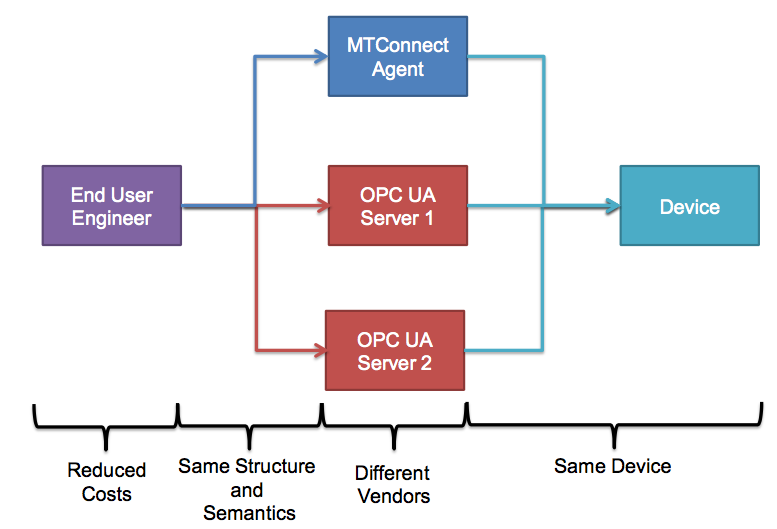
\includegraphics[width=0.75\textwidth]{diagrams/EndUserUseCase.png}
  \caption{End User Engineering Use Case}
  \label{fig:end_user_use_case}
\end{figure}

\section{MTConnect}

\subsection{What is MTConnect?}

MTConnect is an open and royalty-free set of standards designed as a universal factory floor communications protocol. MTConnect is intended specifically for the shop floor environment. While there are numerous communication solutions available, MTConnect defines a “dictionary” for manufacturing data. This means that all data is provided with full context – name, definition, scaling, etc. With most communication networks, all data is defined at the point of use – the application. With MTConnect, the data is defined at the source – the device or Machine Tool. MTConnect devices process information locally and then provide that data in a consistent format to any client application requesting data - ERP, MES, Production Management Systems, Maintenance Systems or a standard Browser, for examples.

\subsection{Basics of MTConnect}

MTConnect is based on standard Internet technologies – HTTP, Ethernet, and XML (Extensible Mark-Up Language – the underlying language of most web sites).
As an Extensible Standard, MTConnect cannot address every conceivable data need on the shop floor. MTConnect provides a clearly defined method for adding additional data types which can be exchanged between equipment, devices, controllers and applications; providing the flexibility to meet the demands of varying environments. 

MTConnect is made up of five fundamental components (see Figure \ref{fig:mtconnect_overview} below):
\begin{itemize}
\item \textbf{Device} -- A type of equipment (Machine Tool) or data source.
\item \textbf{Adapter} -- An optional piece of software (and sometimes hardware) that provides a link or conversion from the data source and data definition in the device to the MTConnect Data definition.  This can be thought of as a translator. The Adapter is not needed for devices that use MTConnect as their native language.
\item \textbf{Agent} -- A piece of software that collects, arranges, and stores data from the device.  It receives requests for data from applications, processes those requests, and then transmits the required data.
\item \textbf{Network} -- The physical connection between a data source (device) and the data consumer (application).  Normally, this is an Ethernet network. The communication on the network normally uses standard internet communications methods – http:// protocol. It should be noted that the MTConnect Structure is adaptable and can be implemented in conjunction with other networking solutions other than Ethernet and Internet protocols.
\item \textbf{Client} -- A Client initiates all requests for MTConnect data. A Client resides in an application or device. The Client is a software function in the application or device that actually requests data from the Agent. 
\end{itemize}

\begin{figure}[h]
  \centering
  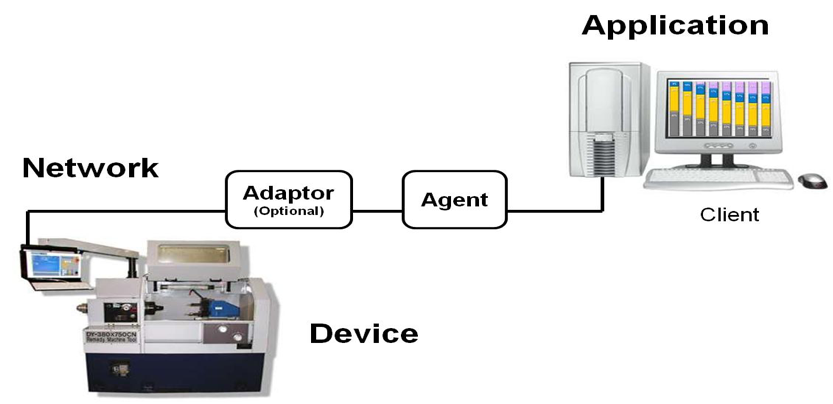
\includegraphics[width=0.75\textwidth]{diagrams/MTConnectOverview.png}
  \caption{MTConnect Overview}
  \label{fig:mtconnect_overview}
\end{figure}

The MTConnect Standard does not restrict the physical implementation of how the MTConnect system is designed.

\begin{itemize}
\item The Network may be a physical implementation, like an Ethernet network. It can also be implemented using wireless or other technologies.
\item The Internet Protocol (http) does not mean that your machine is automatically connected outside your plant to the Internet. This is a communications method only. Protection of your data is controlled by your networking standards. 
\item There is no specific requirement for where the Adaptor and Agent function is located. These can be located at the device. However, they can be placed anywhere in the networking architecture. Also, they do not need to be located together. It is totally MTConnect compliant to have the Adapter installed at the device and the Agent installed along with the Client. The location of these functions should be considered when implementing MTConnect since they will impact the level of data flow on different segments of your network.
\end{itemize}

\section{OPC UA}

\subsection{What is OPC UA?}

OPC UA is an open and royalty free set of standards designed as a universal factory floor communications protocol.
OPC UA is designed specifically for the factory and industrial environment. While there are numerous communication solutions available, OPC UA has several advantages:

\begin{itemize}
\item A state of art security model (see [UA Part 2]).
\item A fault tolerant communication protocol.
\item An information modeling framework that allows application developers to represent their data in a way that makes sense to them.
\end{itemize}

OPC UA has a broad scope which delivers for economies of scale for application developers. This means that a larger number of high quality applications at a reasonable cost are available to factory owners. When combined with powerful semantic models such as MTConnect, OPC UA makes it easier for factory owners to access data via generic commercial application.

The OPC UA model is scalable from small devices to ERP systems. OPC UA devices process information locally and then provide that data in a consistent format to any application requesting data - ERP, MES, PMS, Maintenance Systems, HMI, Smartphone or a standard Browser, for examples. For a more complete overview see [UA Part 1].

\subsection{Basics of OPC UA}

As an Open Standard, OPC UA is based on standard Internet technologies – TCP/IP, HTTP, Ethernet, and XML.

As an Extensible Standard, OPC UA provides a set of services (see [UA Part 4]) and a basic information model framework. This framework provides an easy manner for creating and exposing vendor defined information in a standard way. More importantly all OPC UA Clients are expected to be able to discover and use vendor defined information. This means OPC UA users can benefit from the economies of scale that come with generic visualization and historian applications. This specification is an example of an OPC UA Information Model designed to meet the needs of Machine Tool developers and users.

OPC UA Clients can be any consumer of factory data from another device on the network to browser base thin clients and ERP systems. The full scope of OPC UA applications are shown in Figure \ref{fig:scope_of_opcua}.

The services are described in the following service sets:
\begin{itemize}
\item Discovery Service Set -- used by a Client to discover the Servers and connection information that are available in a system
\item Secure Channel Service Set -- used to establish secure communication over which all subsequent communication occurs. Secure channels specify communication protocols and encoding of data. They are used in conjunction with Session Services and provide consistent functionality for all service sets irrespective of the selected communication protocol (TCP, HTTP, HTTPs) data Encoding (OPC Binary, XML) or network architecture (firewalls, routers \ldots). 
\item Session Service Set -- is used to establish a session context that is used for subsequent communication, including user information. This session context is not lost if a communication error occurs , allowing secure channels to be recovered or rebuilt without data loss
\item \texttt{NodeManagement} Service Set -- allows clients to manage the \texttt{AddressSpace} available in a Server where the \texttt{AddressSpace} is all of the Nodes, both instance and type definition and all of the relationships between them. Management includes adding / deleting nodes and adding / deleting relationships between nodes. Not all Servers support node management functionality.
\item View Service Set – used by a Client to discover the information model that is being exposed in the \texttt{AddressSpace} of the Server It include simple browsing of the address space, but also include services to cover browse information to concrete node references (\texttt{NodeIds})
\item Query Service Set -- is an extension to view service allowing a client to query the \texttt{AddressSpace} of large servers. Usually on large servers support Query services 
\item Attribute Service Set -- allows a client to read and write current and historical values to nodes in the address spaces.
\item Method Service Set -- allow Servers to extend the functionality provided by a system, without having to define new services. The methods are defined in the \texttt{AddressSpace} as part of an information model. Client can discover the available methods using the View Service Set and access them via this service set.
\item \texttt{MonitoredItem} Service Set -- used by client in conjunction with the Subscription Service Set to obtain a steady stream of values. This Service Set allows the client to define the individual data that is to be reported, filters and buffering for the items and the sampling rate.
\item Subscription Service Set -- used by the client in conjunction with the \texttt{Monitored\-Item} Service Set to obtain a steady stream of values. This service set is used to define the grouping of items to be returned and the interval at which they are sent.
\end{itemize}

These standard services are available with any information model, allowing for generic Client access to any Server.

\begin{figure}[h]
  \centering
  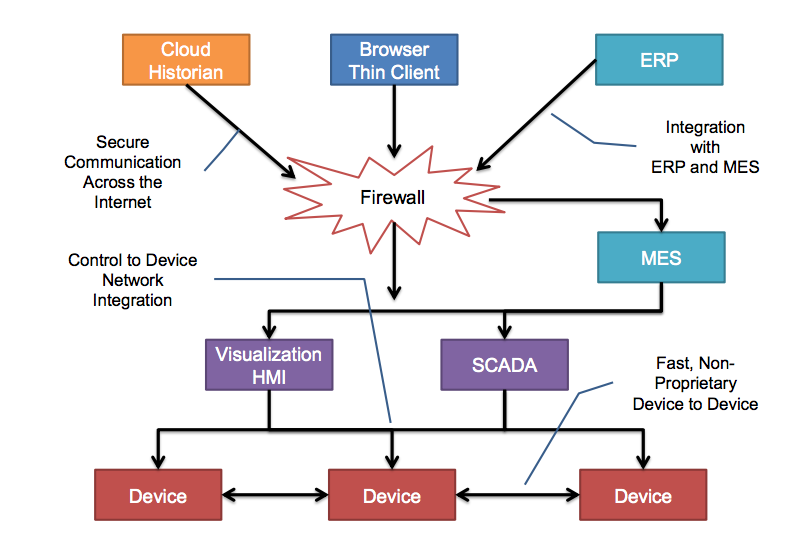
\includegraphics[width=0.85\textwidth]{diagrams/ScopeOfOpcUAEnt.png}
  \caption{The Scope of OPC UA within an Enterprise }
  \label{fig:scope_of_opcua}
\end{figure}

\subsection{Information Modeling in OPC UA}

\subsubsection{Concepts}

OPC UA provides a framework that can be used to represent complex information as Objects in an address space which can be accessed with standard web services. These Objects consist of Nodes connected by References. Different classes of Nodes convey different semantics. For example a Variable Node represents a value that can be read or written. The Variable Node has an associated \texttt{DataType} that can define the actual value, such as a string, float, structure etc. It can also describe the variable value as a variant. A Method Node represents a function that can be called. Every Node has a number of Attributes including a unique identifier called a \texttt{NodeId} and non-localized name called as \texttt{BrowseName}. All of these concepts combined together create what is commonly reference to in OPC UA as the Address Space. An Object representing a 'Reservation' is shown in Figure \ref{fig:opcua_basic_object} as an illustration of these concepts.

\begin{quote}
\footnotesize
NOTE: The figures used to illustrate OPC UA information models use a notation that was developed for the OPC UA specification. The notation is summarized in Figure \ref{fig:opc_ua_notation}. UML representations can also be used; however, the OPC UA notation is less ambiguous because there is a direct mapping from the elements in the figures to Nodes in the address space of an OPC UA server. A complete description of the different types of Nodes and References can be found in [UA Part 3] and the base OPC UA Address space is described in [UA Part 5].
\end{quote}

\begin{figure}[h]
  \centering
  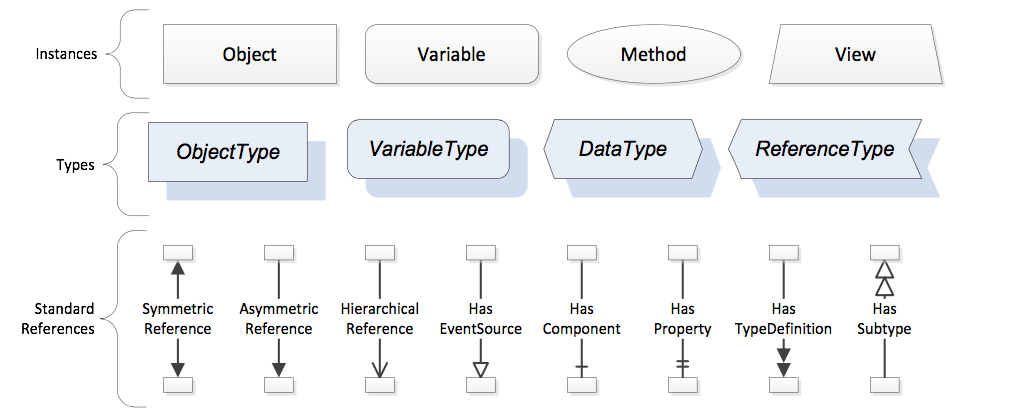
\includegraphics[width=1.0\textwidth]{diagrams/OpcInfoModelNotation.png}
  \caption{The OPC UA Information Model Notation}
  \label{fig:opc_ua_notation}
\end{figure}

\begin{figure}[h]
  \centering
  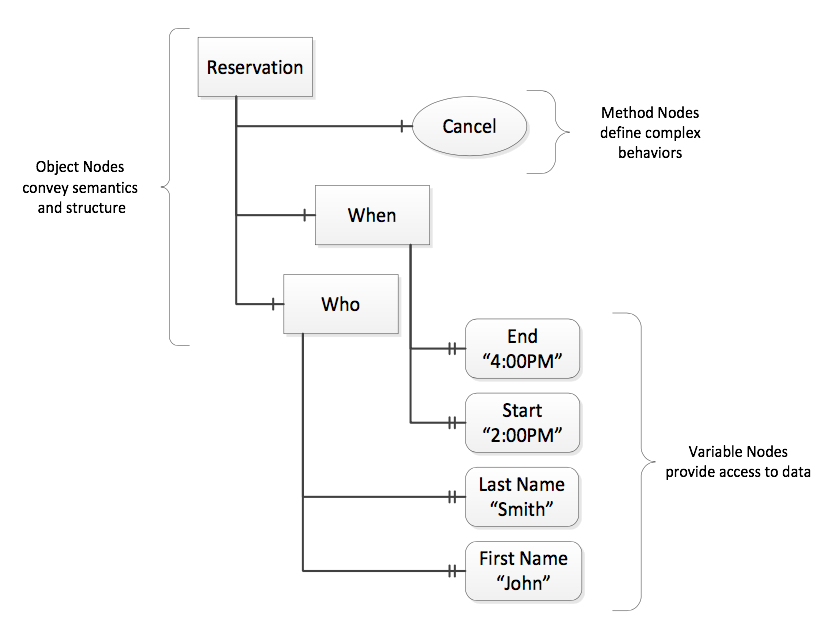
\includegraphics[width=1.0\textwidth]{diagrams/OpcUaBasicObject.png}
  \caption{A Basic Object in an OPC UA Address Space}
  \label{fig:opcua_basic_object}
\end{figure}

\texttt{Object} and \texttt{Variable Nodes} are called \texttt{Instance Nodes} and they always reference a Type Definition (\texttt{ObjectType} or \texttt{VariableType}) Node which describes their semantics and structure. Figure \ref{fig:rel_type_inst} illustrates the relationship between an Instance and its Type Definition.

The Type Nodes are templates that define all of the children that can be present in an Instance of the Type. In the example in Figure \ref{fig:rel_type_inst} the \texttt{PersonType} \texttt{ObjectType} defines two children: First Name and Last Name. All instances of \texttt{PersonTyp}e are expected to have the same children with the same \texttt{BrowseNames}. Within a Type the \texttt{BrowseNames} uniquely identify the child. This means Client applications can be designed to search for children based on the \texttt{BrowseNames} from the Type instead of \texttt{NodeIds}. This eliminates the need for manual reconfiguration of systems if a Client uses Types that multiple devices implement.

OPC UA also supports the concept of sub typing. This allows a modeler to take an existing Type and extend it. There are rules regarding sub typing defined in [UA Part 3], but in general they allow the additions to a given type or the restriction of a \texttt{DataType} to a more specific data type. For example the modeler may decide that the existing \texttt{ObjectType} in some cases needs an additional variable. The modeler can create a subtype of the \texttt{ObjectType} and add the variable. A client that is expecting the parent type can treat the new \texttt{ObjectType} as if it was of the parent \texttt{ObjectType} and just ignore the additional variable. A client that understands the new subtype may display or otherwise process the additional variable. With regard to \texttt{DataTypes}, if a variable is defined to have a numeric value, a sub type could restrict the Value to a float.

\begin{figure}[h]
  \centering
  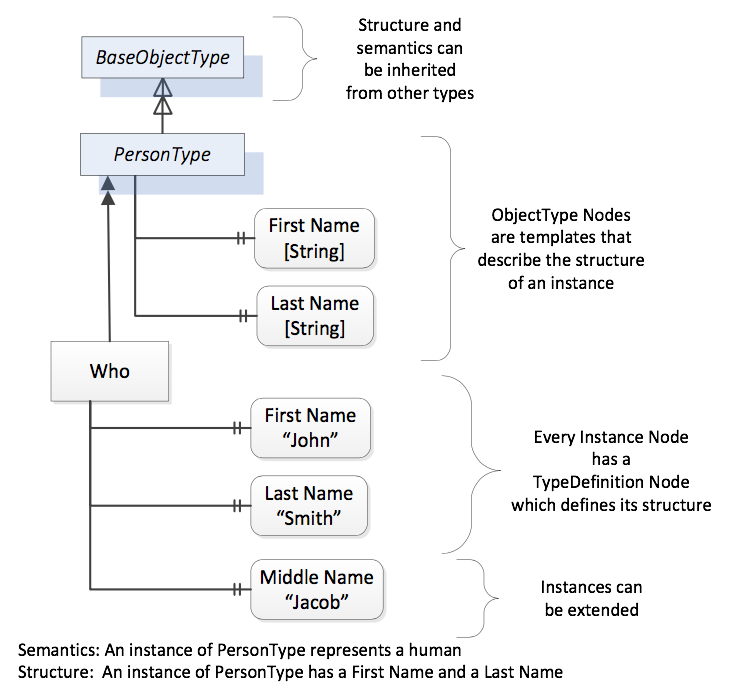
\includegraphics[width=1.0\textwidth]{diagrams/RelsBetweenTypesAndInstances.png}
  \caption{The Relationship between Type Definitions and Instances }
  \label{fig:rel_type_inst}
\end{figure}

References allow Nodes to be connected together in ways that describe their relationships. All References have a ReferenceType that specifies the semantics of the relationship. References can be hierarchical or non-hierarchical. Hierarchical references are used to create the structure of Objects and Variables. Non-hierarchical are used to create arbitrary associations. Applications can define their own ReferenceType by creating Subtypes of the existing ReferenceType. Subtypes inherit the semantics of the parent but may add additional restrictions. Figure \ref{fig:ref_bet_objs} depicts several references connecting different Objects.

\begin{figure}[h]
  \centering
  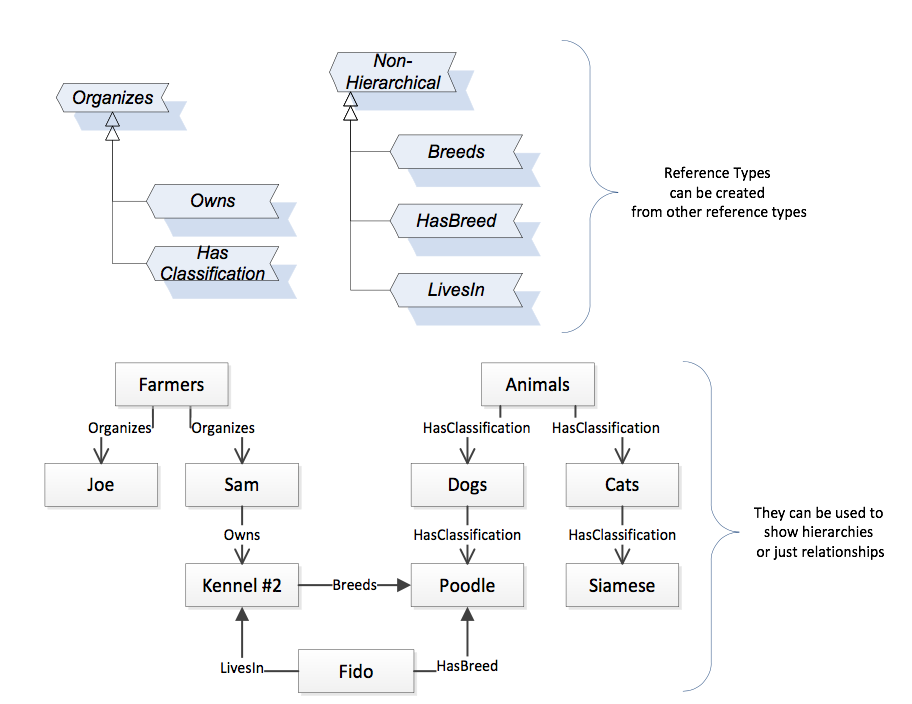
\includegraphics[width=1.0\textwidth]{diagrams/RefsBetweenObjects.png}
  \caption{Examples of References between Objects}
  \label{fig:ref_bet_objs}
\end{figure}

OPC UA specification defines a very wide range of functionality in its basic information model. It is not expected that all clients or servers support all functionality in the OPC UA specifications. OPC UA includes the concept of profiles, which segment the functionality into testable certifiable units. This allows the development of companion specification (such as MTConnect-OPC UA) that can describe the subset of functionality that is expected to be implemented. The profiles do not restrict functionality, but generate requirements for a minimum set of functionality (see [UA Part 7])

The OPC foundation also defines a set of information models that provide a basic set of functionality. The Data Access specification (see [UA Part 8]) provides a basic information model for typical data. The Alarm and Condition specification (see [UA Part 9]) defines a standard information model for Alarms and Conditions. The Programs specification (see [UA Part 10]) defines a stand information model for extending the functionality available via method calls and state machines. The Historical Access specification (see [UA Part 11]) defines the information model associated with Historical Data and Historical Events. The aggregates specification (see [UA Part 13]) defines a series of standard aggregate function that allow a client to request summary data. Examples of aggregates include averages, minimums, time in state, Standard deviation, etc. 

\subsubsection{Namespaces}

OPC UA allows information from many different sources to be combined into a single coherent address space. \texttt{Namespaces} are used to make this possible by eliminating naming and id conflicts between information from different sources. \texttt{Namespaces} in OPC UA have a globally unique string called a \texttt{NamespaceUri} and a locally unique integer called a \texttt{NamespaceIndex}. The \texttt{NamespaceIndex} is only unique within the context of a Session between an OPC UA Client and an OPC UA Server. All of the web services defined for OPC UA use the \texttt{NamespaceIndex} to specify the \texttt{Namespace} for qualified values.

There are two types of values in OPC UA that are qualified with Namespaces: \texttt{NodeIds} and \texttt{QualifiedNames}. \texttt{NodeIds} are globally unique identifiers for Nodes. This means the same Node with the same \texttt{NodeId} can appear in many Servers. This, in turn, means Clients can have built in knowledge of some Nodes. OPC UA Information Models generally define globally unique \texttt{NodeIds} for the \texttt{TypeDefinitions} defined by the Information Model.

\texttt{QualifiedNames} are non-localized names qualified with a \texttt{Namespace}. They are used for the \texttt{BrowseNames} of Nodes and allow the same Names to be used by different information models without conflict. The \texttt{BrowseName} is used to identify the children within a \texttt{TypeDefinitions}. Instances of a \texttt{TypeDefinition} are expected to have children with the same \texttt{BrowseNames}. \texttt{TypeDefinitions} are not allowed to have children with duplicate \texttt{BrowseNames}; however, Instances do not have that restriction.

\subsubsection{Companion Specifications}

An OPC UA companion specification for an industry specific vertical market describes an information model by defining ObjectTypes, VariableTypes, DataTypes and ReferenceTypes that represent the concepts used in the vertical market. Table \ref{table:ex_object_type_definition} contains an example of an ObjectType definition.

\begin{table}[ht]
\centering 
  \caption{Example \texttt{ObjectType} Definition}
  \label{table:ex_object_type_definition}
\fontsize{9pt}{11pt}\selectfont
\tabulinesep=3pt
\begin{tabu} to 6in {|l|l|l|l|l|l|} \everyrow{\hline}
\hline
\rowfont\bfseries {Attribute} & \multicolumn{5}{|l|}{Value} \\
\tabucline[1.5pt]{}
BrowseName & \multicolumn{5}{|l|}{WidgetType} \\
IsAbstract & \multicolumn{5}{|l|}{True} \\
\tabucline[1.5pt]{}
\rowfont \bfseries References & NodeClass & BrowseName & DataType & TypeDefinition & {Modeling Rule} \\
\multicolumn{6}{|l|}{Subtype of the BaseObjectType from [UA Part 5]} \\
HasProperty & Variable & Color &  String & PropertyType & Optional \\
HasProperty & Variable & Flavor &  Double & PropertyType & Mandatory \\
HasProperty & Variable & Rank &  Int32 & PropertyType & Mandatory \\
\end{tabu}
\end{table} 

The \texttt{BrowseName} is a non-localized name for an \texttt{ObjectType}. 

\texttt{IsAbstract} is a flag indicating whether instances of the \texttt{ObjectType} can be created.

The bottom of the table lists the child nodes for the type. The Reference is the type of reference between the Object instance and the child Node. The \texttt{NodeClass} is the class of Node. The \texttt{BrowseName} is the non-localized name for the child. The \texttt{DataType} is the structure of the Value accessible via the Node (only used for Variable \texttt{NodeClass} Nodes) and the \texttt{TypeDefinition} is the \texttt{ObjectType} or \texttt{VariableType} for the child. 

The \texttt{ModellingRule} indicates whether a child is Mandatory or Optional. It can also indicate cardinality. Note that the \texttt{BrowseName} is not defined if the cardinality is greater than 1. Figure \ref{fig:sample_object_type} visually depicts the \texttt{ObjectType} defined in Table \ref{table:ex_object_type_definition} along with two instances of the \texttt{ObjectType}.

\begin{figure}[h]
  \centering
  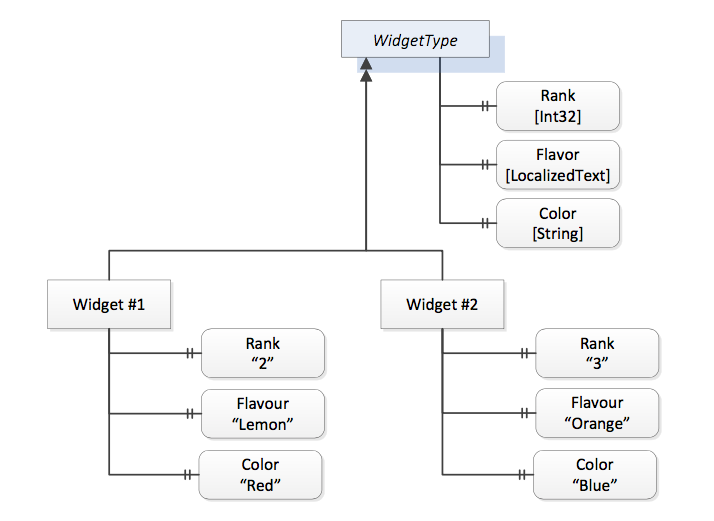
\includegraphics[width=1.0\textwidth]{diagrams/SampleObjectType.png}
  \caption{A Visual Representation of the Sample ObjectType}
  \label{fig:sample_object_type}
\end{figure}

\FloatBarrier
\section{MTConnect in OPC UA}

\begin{quote}
    \color{red}
    Todo: This section will need to be rewritten with the new activity and data flow models and the factories to create the information models.
\end{quote}

\subsection{Base Information}

It is expected that MTConnect and OPC UA will continue to evolve their respective standards, in particular as the MTConnect defined information model is revised an OPC UA Client may desire to know the version of the MTConnect model implement by a given server. The information model will always be backwards compatible.

MTConnect defines a Probe request, which is just mapped to an OPC UA Browse. The Probe request returns the devices that are defined in an agent. In OPC UA, a client can at any time browse the address space, and return the detailed structure of the address space, this includes all relationships between devices, their defined types and data types. An OPC UA Client can also subscribe for a \texttt{ModelChangeEvents} changes and \texttt{SemanticChangeEvents} which allow the client to be notified if the address space is modified. \texttt{ModelChangeEvent} are generated by server whenever a new node or reference is added to a server. The Node may be a new type definition, change to a type definition or a new instance node. \texttt{SemanticChangeEvents} are generated by a server when some aspect of an instance of a node type is change and the change would result in a change that a client should be aware of. An example of a \texttt{SemanticChangeEvent} would be for a change in the engineering Unit assigned to a node.

MTConnect defines a Sample Request command to obtain information from the device. This command can be mapped to an OPC UA read or subscription service. The read service will return the latest value of the requested item. This is appropriate for obtaining the most recent value of a variable. The Subscription service is described the next paragraph. In some cases Historical data access may be required. This allows a client to obtain older values for a device, based on time ranges or other criteria. This feature can be used by a server to allow addition data to be available and could be used to enhance MTConnect Sample Request for cases where more than just the current value is required.

MTConnect describes a Streaming command, which matches to the OPC UA subscription service. This service would allow a client to obtain a steady stream of values associated with a device. The subscription service supports filtering, based on data changes or even aggregates, where an aggregate is a minimum, maximum, average, time in state or any of a long list of aggregates. For a complete list of OPC defined aggregates see [UA Part 11]. It would also allow the return of any OPC Events associated with the device. An OPC Event in MTConnect terms would be a transition of a Condition. Subscription data includes message information that allows a client to determine if a packet was missed or is out of order. The client can request a replay of any missed information or re-sequence the packets. Also included is a keep-alive heart beat that allows for rapid determination of and recovery from communication failures. This functionality is used to ensure the MTConnect Streaming functionality is matched.

MTConnect defines Asset, which becomes a simple addition to the OPC UA information model that describes the MTConnect devices. MTConnect defines the structure of many standard devices, components or Asset. The remainder of this document will provide a mapping of the information model that is described by mapping these MTConnect items into an OPC UA information model.

MTConnect error codes will be mapped to OPC UA error codes where appropriate. The OPC UA server has a multilevel error reporting capability. A Service can include  	 information, as well as the individual data items that are being reported as part of the service.

As discussed in the overview of OPC UA, all companion specifications usually define a \texttt{Namespace}. For this companion specification all \texttt{Type\-Definitions} and \texttt{Browse\-Names} defined by this specification are qualified by the MTConnect \texttt{Namespace} \\
\texttt{("urn:mtconnect.com:MTConnectDevices:1.2")} unless stated otherwise.

The description associated with MTConnect items is always mapped to the Description attribute available in OPC UA.

The Name from MTConnect is always mapped to the BrowseName in OPC UA.

The \texttt{NativeName} from MTConnect will be the \texttt{DisplayName}, but if a \texttt{NativeName} is not provided then the \texttt{BrowseName} will be used as the default DisplayName.

The \texttt{UUID} from \texttt{MTConnect} can be mapped to the \texttt{NodeId} in OPC UA. The Namespace associated with MTConnect will assure that the \texttt{NodeId} is unique.

\FloatBarrier
\subsection{Additional Subscription Information}

A \texttt{DataChange} Subscription can be created with the following steps:

\begin{itemize}
\item Browse the Address Space and read the NodeIds for the DataItems of interest;
\item Create a Subscription;
\item Create a MonitoredItem for each DataItem of interest;
\end{itemize}

As an alternative to browsing the address space, a browse path from a starting node can be created using the type definitions and the \texttt{TranslateBrowsePathsToNodeIds} service can be called to obtain the actual \texttt{NodeIds}. Figure \ref{fig:browse_path_ex} provides an example of a data item that is for a know type. The illustrated path is the same for any instance of a boiler object.

\begin{figure}[h]
  \centering
  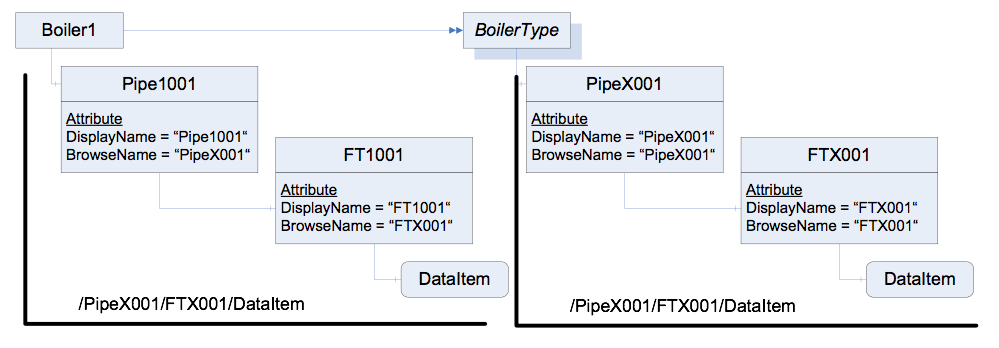
\includegraphics[width=1.0\textwidth]{diagrams/BrowsePathEx.png}
  \caption{Browse Path Example}
  \label{fig:browse_path_ex}
\end{figure}

Each Notification has the current value for a \texttt{DataItem}, the \texttt{Timestamp} and \texttt{Status\-Code}.

The \texttt{MonitoredItem} allows the Client to specify a different SamplingInterval and \texttt{QueueSize} for each \texttt{DataItem}. The \texttt{MinimumSamplingInterval} attribute for each \texttt{DataItem} specifies the fastest supported \texttt{SamplingInterval}. The \texttt{Publishing\-Interval} for a Subscription controls how frequently Notifications are returned to the Client. If this value is longer than \texttt{Sampling\-Interval} then the Server will buffer changes and return multiple Notifications in one message. 

An OPC \texttt{Event} Subscription can be created with the following steps: 

\begin{itemize}
\item Browse the Address Space and read the \texttt{NodeIds} for the Devices or \texttt{Components} of interest;
\item Create a Subscription;
    \begin{itemize}
    \item Create a \texttt{MonitoredItem} for each Device or Component of interest;
    \item Select the fields to return for each event, where the complete list of available fields is defined as part of the OPC UA \texttt{EventType} definition;
    \item Specify additional filter criteria for the events to return; 
    \end{itemize}
\end{itemize}

Events in OPC UA propagate up the \texttt{HasNotifier} hierarchy. This means subscribing to a parent Node in a hierarchy (i.e. an MTConnect Device) will request events for all Components under that Node. If a Client wants to receive all events for all devices it can subscribe to the Server node.
Each Condition Event is a snapshot of the \texttt{MTConditionType} Object. The Client must select the fields from the Condition that it wishes to receive in the update by specifying the \texttt{BrowsePath} (a sequence of \texttt{BrowseNames}). 

\begin{quote}
    \color{red}
    TODO: Need to provide model of event and condition management in MTConnect. Activity Models will be added here..
\end{quote}

\clearpage

\section{MTConnect Devices}\label{mtconnect_devices}
\FloatBarrier

\input ./types.tex

\end{document}
